\newpage
\subsection{Melihat Daftar Barang yang Dillang}
Halaman ini hanya dapat diakses oleh pengguna yang sudah terdaftar dan sudah \textit{login} ke dalam sistem. Halaman ini menampilkan \textit{form} berisi elemen \textit{input} data diri, dan pengguna dapat mengisi lalu mengklik tombol daftar, dan untuk kasus normal dan alternatif dapat dilihat pada Tabel \ref{uc02.01}.\\
\indent Terdapat \textit{view logic} khusus pada halaman ini yang ditulis menggunakan Vue dan di\textit{compile} dengan menggunakan webpack, yang akan dicantumkan dalam Kode Sumber \ref{cdv.02-01}. Kode sumber implementasi \textit{back-end} dapat dilihat pada Kode Sumber \ref{cdbe.02-01}.

\begin{lstlisting}[label=cdbe.02-01,style=php,caption=Implementasi \textit{Back-end} Melihat Daftar Barang]
/*	file : app/Http/Controllers/HomeController*/
 public function index(){
	 /*	method : GET */
	 
	 /*	variabel berisi id barang 
		yang disort dari tanggal perbaruan
		secara descending */
	 $data['items'] = Item::all()->sortByDesc('created_at');
	 
	 /*	variabel berisi id barang 
		 yang sedang aktif proses lelang
		 menggunakan repository : itemRepository */
	 $data['activebid'] = $this->itemRepository->getActiveItem();
	 

	 return view('pages.general.landing', $data);
 }
\end{lstlisting}

\begin{lstlisting}[label=cdv.02-01,style=htmlcssjs,caption=Implementasi Vue Melihat Daftar Barang]
<div>
	 <img :src="imgUrl"  class="img-responsive" />
	 
	 <div class="ribbon" v-if="isFavorited" @click.prevent="unFavorite(item)" >
		 <div class="border-ribbon"></div>
		 <i class="fa fa-heart"></i>
	 </div>
	 
	 <div class="unribbon" v-else @click.prevent="favorite(item)">
		 <div class="border-ribbon"></div>
		 <i class="fa fa-heart-o"></i>
	 </div>
</div>

export default {
    props: ['item', 'favorited'],
    data: function() {
        return {
            isFavorited: '',
            imgUrl : 'http://URL_GAMBAR_DEFAULT'
        }
    },
    mounted() {
        this.isFavorited = this.isFavorite ? true : false;
    },
    created() {
        axios.get("get/img/item/" + this.item)
            .then( response => {
	            if(response.data.replace(/\s+/g, '') != '' ){
	            	var url =  /*rewrite image url*/;
	            	this.imgUrl = url.replace(/\s+/g, '');
	            	console.log(this.imgUrl);
	        	}
    	});
    },
    computed: {
        isFavorite()
        {
            return this.favorited;
        }
    },
    methods: {
        favorite(item){
            axios.post('/ajax/favourite/'+item)
                .then(response => this.isFavorited = true)
        		.catch(response => console.log(response.data));
        	},
        unFavorite(item) {
            axios.post('/ajax/favourite/un/'+item)
                .then(response => this.isFavorited = false)
        		.catch(response => console.log(response.data));
        }
    }
}
\end{lstlisting}

\begin{figure}[H]
	\centering
	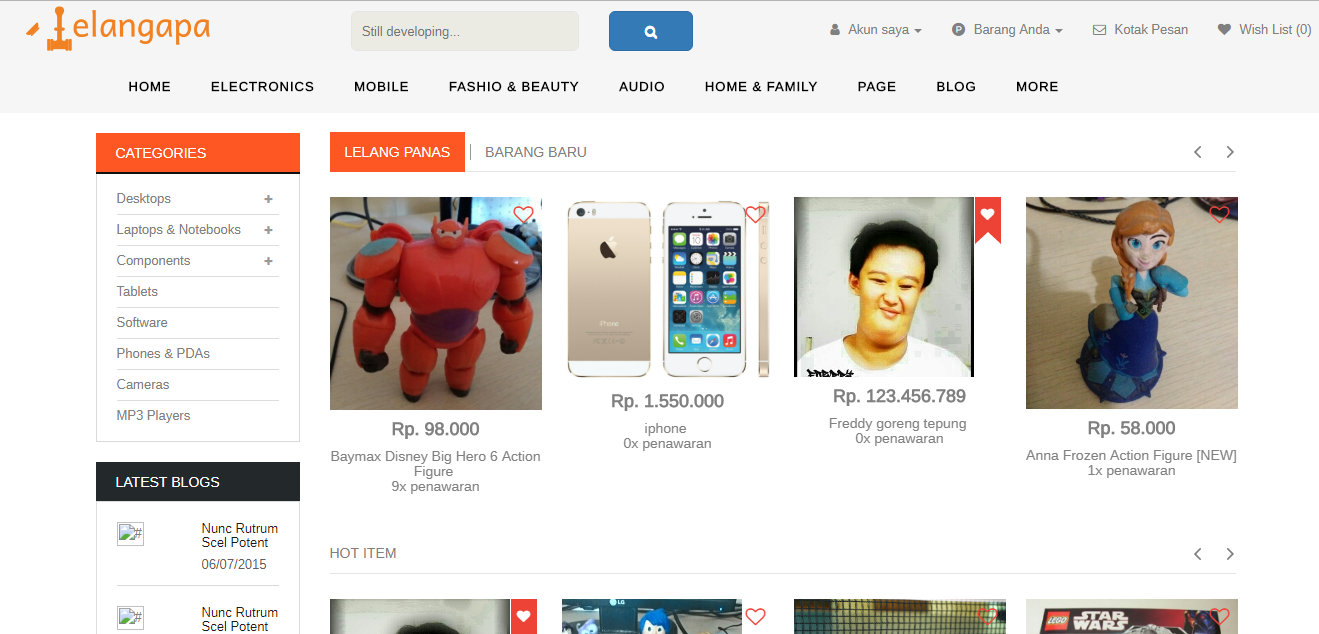
\includegraphics[width=\textwidth]{images/bab4/ui/02-01.png}
	\caption{Halaman Antarmuka Melihat Barang yang Dilelang }
	\label{ui.02-01}
\end{figure}

